\newpage
\section{File and directory}

% Chiamata stat()
\subsection{Chiamata stat()}

Legge l'inode e ti fornisce i \hl{dati che puoi sapere riferiti a quell'inode}. Tramite il comando \hl{dumpe2fs} che fa il \hl{dump di tutta la struttura dati nella partizione designata}.

Se vogliamo \hl{trovare i puntatori ed i blocchi di un file dato il suo nome andiamo a guardare l'inode}, troviamo i blocchi che gli appartengono e poi tramite il comando \hl{dd} possiamo andare \hl{tagliare i blocchi nel file che rappresenta la nostra partizione} dove ci saranno da rispettare alcune regole sul quanti byte rappresentano un blocco ecc (regole del file system).

La funzione stat prende come \hl{parametri}:

\begin{lstlisting}
int stat(const char *restrict pathname, struct stat *restrict buf);
\end{lstlisting}

con:

\begin{itemize}
    \item \hl{path}: del quale dire i dati
    \item \hl{struct}: parametri di uscita dato che è un puntatore
\end{itemize}


Le sue \hl{varianti} sono:

\begin{itemize}
    \item \hl{fstat}: usa un \textbf{fd al posto del path}
    \item \hl{lstat}: prende dei \textbf{link simbolici} in pathname (può esser usata anche per file normali)
    \item \hl{fstatat}: prende \textbf{sia un fd che un pathname}
\end{itemize}

Nella \hl{struttura stat} abbiamo tutti i dati come output dalla funzione:

\begin{lstlisting}
struct stat {
	mode_t		st_mode;	/*file type & mode (permissions)*/
	ino_t		st_ino;		/*i-node number (serial number)*/
	dev_t		st_dev;		/*device number (file system)*/
	dev_t		st_rdev;	/*device number for special files*/
	nlink_t		st_nlink;	/*number of links*/
	uid_t		st_uid;		/*user ID of owner*/
	gid_t		st_gid;		/*group ID of owner*/
	off_t		st_size;	/*size in bytes, for regular files*/
	struct timespec st_atim;/*time of last access*/
	struct timespec st_mtim;/*time of last modification*/
	struct timespec st_ctim;/*time of last file status change*/
	blksize_t	st_blksize;	/*best I/O block size*/
	blkcnt_t	st_blocks;	/*number of disk blocks allocated*/
};
\end{lstlisting}

dove \hl{st\_mode contiene sia il tipo di file che i privilegi}. Per vedere che file è ci sono delle \hl{function like macro}:

\begin{table}[!h]
	\centering
	\begin{tabular}{|c|c|}
		\hline
		\textbf{Macro} & \textbf{Type of file} \\\hline\hline
		S\_ISREG() & regular file \\
		S\_ISDIR() & directory file \\
		S\_ISCHR() & character special file \\
		S\_ISBLK() & block special file \\
		S\_ISFIFO() & pipe or FIFO \\
		S\_ISLNK() & symbolic link \\
		S\_ISSOCK() & socket \\\hline
	\end{tabular}
	\caption{\label{tab:widgets}File type macros in <sys/stat.h>}
\end{table}

è un'esempio di check del tipo di file il file filetype.c:

\begin{lstlisting}
#include "apue.h"

int
main(int argc, char *argv[])
{
	int			i;
	struct stat	buf;
	char		*ptr;

	for (i = 1; i < argc; i++) {
		printf("%s: ", argv[i]);
		if (lstat(argv[i], &buf) < 0) {
			err_ret("lstat error");
			continue;
		}
		if (S_ISREG(buf.st_mode))
			ptr = "regular";
		else if (S_ISDIR(buf.st_mode))
			ptr = "directory";
		else if (S_ISCHR(buf.st_mode))
			ptr = "character special";
		else if (S_ISBLK(buf.st_mode))
			ptr = "block special";
		else if (S_ISFIFO(buf.st_mode))
			ptr = "fifo";
		else if (S_ISLNK(buf.st_mode))
			ptr = "symbolic link";
		else if (S_ISSOCK(buf.st_mode))
			ptr = "socket";
		else
			ptr = "** unknown mode **";
		printf("%s\n", ptr);
	}
	exit(0);
}	
\end{lstlisting}


% User-ID e Group-ID
\subsection{User-ID e Group-ID}

\hl{Ogni processo ha piu' ID associati} a lui:

\begin{itemize}
	\item \hl{real user/group ID}: indica chi siamo
	\item \hl{effective user/group ID}: usato quando c'è il set user id attivo e si \textbf{presenta come proprietario del file} e potrà quindi leggerlo, scriverlo ecc
	\item supplementary group ID: quando un utente è stato aggiunto ad un gruppo
	\item \hl{saved set-user/group-ID}: sono delle identità associate ad un processo e fa si che \textbf{se è stato root} e lascia i privilegi \textbf{potrà riconquistarli}
\end{itemize}

I permessi saranno verificabili tramite delle macro che hanno accesso un solo bit:

\begin{table}[!h]
	\centering
	\begin{tabular}{|c|c|}
		\hline
		\textbf{st\_mode mask} & \textbf{Meaning} \\\hline\hline
		S\_IRUSR & user-read \\
		S\_IWUSR & user-write \\
		S\_IXUSR & user-execute \\\hline
		S\_IRGRP & group-read \\
		S\_IWGRP & group-write \\
		S\_IXGRP & group-execute \\\hline
		S\_IROTH & other-read \\
		S\_IWOTH & other-write \\
		S\_IXOTH & other-execute \\\hline
	\end{tabular}
	\caption{\label{tab:widgets}The nine file access permission bits, from <sys/stat.h>}
\end{table}


Notare che \hl{per eliminare un file esistente} non ci vuole il permesso di scrittura sul file ma il \hl{permesso di srittura sulla directory} dato che stai scrivendo la directory.

Grazie alle ACL (sono delle estenzioni) possiamo dare il permesso al file e dire che non può essere cancellato da un utente specifico o meno. Usiamo l'opzione:

\begin{lstlisting}
ls -le file
\end{lstlisting}

Il test di accesso al file che il kernel esegue quando si lavroa conun file dipende dal proprietario del file. Il test sono:

\begin{itemize}
	\item effective user ID = 0: ...
	\item effective user ID = owner ID: ... se non c'è il permesso ma lo ha il gruppo allora non potrò accederci dato che il test guarda user e poi group (in pratica non viene proprio guardato)
\end{itemize}


% Funzioni access() e faccessat()
\subsection{Funzioni access() e faccessat()}

\hl{Dice in anticipo se si puo' o no fare una cosa}. Il processo ha i suoi ID ed in base ai permessi potrà, o no, fare delle operazioni. Usiamo questa funzione:

\begin{lstlisting}
int access(const char *pathname, int mode);
\end{lstlisting}

con mode:

\begin{table}[!h]
	\centering
	\begin{tabular}{|c|c|}
		\hline
		\textbf{mode} & \textbf{Description} \\\hline\hline
		R\_OK & test for read permission \\
		W\_OK & test for write permission \\
		X\_OK & test for execute permission \\\hline
	\end{tabular}
	\caption{\label{tab:widgets}The mode flags for access function, from <unistd.h>}
\end{table}


% Funzione umask()
\subsection{Funzione umask()}

Mostra in ottale i \hl{privilegi che verrano tolti al file} in merito a lettura e scrittura:

\begin{lstlisting}
mode_t umask(mode_t mask);
\end{lstlisting}

viene \hl{ereditata dai processi} data la loro possiblità di creare file.

Su linux la troviamo in:

\begin{lstlisting}
$ cat /proc/$$/status
...
Umask:		0022
...
\end{lstlisting}


% Sticky bit
\subsection{Sticky bit}

Permesso che ha senso per le cartelle \hl{quando piu' persone ci lavorano}, ma senza che un utente possa eliminare file che non gli appartengono.

\begin{lstlisting}
drwxrwxrwt  15 root  wheel   480 Oct 14 22:00 Shared
\end{lstlisting}

la stessa cosa esiste per le cartelle temporanee.


% File truncation
\subsection{File truncation}

È possibile da file \hl{tagliare una parte di file} esprimendo la lunghezza:

\begin{lstlisting}
int truncate(const char *pathname, off_t length); 
int ftruncate(int fd, off_t length);
\end{lstlisting}


% Hard link e link simbolici
\subsection{Hard link e link simbolici}

La \hl{funzione} per crearli in C è:

\begin{lstlisting}
int link(const char *existingpath, const char *newpath);
int linkat(int efd, const char *existingpath, int nfd, const char *newpath, int flag);
\end{lstlisting}

Abbiamo delle funzioni che seguiranno i link simbolici ed altre che seguiranno direttamente il file:


\begin{table}[!h]
    \centering
    \begin{tabular}{|c|c|c|}
        \hline
        \textbf{Function} & \textbf{Does not follow symbolic link} & \textbf{Follows symbolic link} \\\hline\hline
        access &  & $\bullet$ \\\hline
        chdir &  & $\bullet$ \\\hline
        chmod &  & $\bullet$ \\\hline
        chown &  & $\bullet$ \\\hline
        creat &  & $\bullet$ \\\hline
        exec &  & $\bullet$ \\\hline
        lchown & $\bullet$ &  \\\hline
        link &  & $\bullet$ \\\hline
        lstat & $\bullet$ &  \\\hline
        open &  & $\bullet$ \\\hline
        opendir &  & $\bullet$ \\\hline
        pathconf &  & $\bullet$ \\\hline
        readlink & $\bullet$ &  \\\hline
        remove & $\bullet$ &  \\\hline
        rename & $\bullet$ &  \\\hline
        stat &  & $\bullet$ \\\hline
        truncate &  & $\bullet$ \\\hline
        unlink & $\bullet$ & \\\hline
    \end{tabular}
    \caption{\label{tab:widgets}Tabella delle funzioni}
\end{table}


Tramite i link simbolici è possibile \hl{creare dei loop} nei quali l'OS si può bloccarsi. 


\begin{figure}[H]
\centering
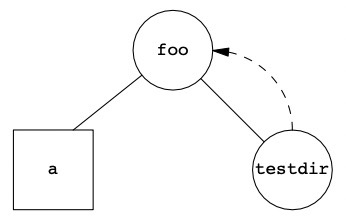
\includegraphics[scale=0.4]{linkloop.jpeg}
\caption{Loop generato da un link simbolico} 
\label{linkloop}
\end{figure}


Per i \hl{link simbolici} usiamo le funzioni:

\begin{itemize}
	\item \hl{symlink()}: crea un link simbolico

\begin{lstlisting}
int symlink(const char *actualpath, const char *sympath);
\end{lstlisting}

	\item \hl{readlink()}: combina le azioni di apertura, lettura e chiusura

\begin{lstlisting}
ssize_t readlink(const char* restrict pathname, char *restrict buf,size_t bufsize);
\end{lstlisting}

\end{itemize}


% File times
\subsection{File times}

Abbiamo 3 tipi di file times:

\begin{table}[!h]
    \centering
    \begin{tabular}{|c|c|c|}
        \hline
        \textbf{Field} & \textbf{Description} & \textbf{Example} \\\hline\hline
        st\_atim & last-access time of file data & read \\\hline
        st\_mtim & last-modification time of file data & write \\\hline
        st\_ctim & last-change time of i-node status & chmod, chown \\\hline
    \end{tabular}
    \caption{\label{tab:widgets}The three time values associated with each file}
\end{table}


Esistono delle funzioni per poter \hl{modificare i tempi}:

\begin{itemize}
	\item \hl{futimens}: dove "f" sta per fd, invece "u" per nanosecondi

\begin{lstlisting}
int futimes(int fd, const struct timespec times[2]);
\end{lstlisting}

\begin{itemize}
	\item \textbf{fd}: file scriptor, quindi cambi il tempo ad un file già aperto
	\item \textbf{times[2]}: array con tempo di accesso e di modifica che a loro volta sono composti da più campi dato che sono di tipo timespec
\end{itemize}

	\item \hl{utimensat}: uguale a futimens ma usa i \textbf{microsecondi}, che sono meno affidabili detti da un compilatore dato che la granularità promessa è minore di quella possibile
	
\begin{lstlisting}
int utimensat(int fd, const char *pathname, const struct timespec times[2], int flag);
\end{lstlisting}

	\item \hl{utimes}
\end{itemize}

o più semplicemente abbiamo "touch" che ci permette di modificare il tempo di accesso:

\begin{lstlisting}
$ stat -x prova
...
Access: Fri Oct 21 16:54:30 2022
Modify: Fri Oct 21 16:54:30 2022
Change: Fri Oct 21 16:54:30 2022
 Birth: Fri Oct 21 16:54:30 2022

$ touch prova
$ stat -x prova
...
Device: 1,18   Inode: 28513966    Links: 1
Access: Fri Oct 21 16:55:06 2022
Modify: Fri Oct 21 16:55:06 2022
Change: Fri Oct 21 16:55:06 2022
 Birth: Fri Oct 21 16:54:30 2022
\end{lstlisting}


Per capire come funziona possiamo analizzare il file zap.c:

\begin{lstlisting}
#include "apue.h"
#include <fcntl.h>

int
main(int argc, char *argv[])
{
	int				i, fd;
	struct stat		statbuf;
	struct timespec	times[2];

	for (i = 1; i < argc; i++) {
		if (stat(argv[i], &statbuf) < 0) {	/* fetch current times */
			err_ret("%s: stat error", argv[i]);
			continue;
		}
		if ((fd = open(argv[i], O_RDWR | O_TRUNC)) < 0) { /* truncate */
			err_ret("%s: open error", argv[i]);
			continue;
		}
		times[0] = statbuf.st_atim; /* per MacOS usare st_atimeprec */
		times[1] = statbuf.st_mtim; /* per MacOS usare st_mtimeprec */
		if (futimens(fd, times) < 0)		/* reset times */
			err_ret("%s: futimens error", argv[i]);
		close(fd);
	}
	exit(0);
}
\end{lstlisting}

dove:

\begin{itemize}
	\item \hl{if 1}: leggo il file e lo metto nella \textbf{struttura nel buffer}
	\item \hl{if 2}: effettuo una qualsiasi modifica, in questo caso un troncamento
	\item \hl{times[...]}: carico i vecchi tempi
	\item \hl{if 3}: resetta i tempi del file a quelli iniziali
\end{itemize}

notiamo però che la modifica non può intaccare anche il tempo di change non viene mai risettato a quello originare dato che \hl{non puo' essere toccato}:

\begin{lstlisting}
$ touch prova
$ stat -x prova
...
Access: Fri Oct 21 17:11:28 2022
Modify: Fri Oct 21 17:11:28 2022
Change: Fri Oct 21 17:11:29 2022
 Birth: Fri Oct 21 17:11:28 2022

$ ./zap prova
$ stat -x prova
...
Access: Fri Oct 21 17:11:28 2022
Modify: Fri Oct 21 17:11:28 2022
Change: Fri Oct 21 17:12:07 2022
 Birth: Fri Oct 21 17:11:28 2022
\end{lstlisting}


% Reading directories
\subsection{Reading directories}

Abbiamo vari modi per leggere delle directory:

\begin{itemize}
	\item opendir:

\begin{lstlisting}
DIR *opendir(const char *pathname);
\end{lstlisting}

	\item \hl{fdopendir}: per \textbf{aprire una directory tramite fd}

\begin{lstlisting}
DIR *fdopendir(int fd); 
\end{lstlisting}

	\item \hl{readdir}: si posiziona nel \textbf{leggere il file successivo} della directory

\begin{lstlisting}
struct dirent *readdir(DIR *dp); 
\end{lstlisting}

	\item \hl{rewinddir}: riposiziona il \textbf{cursore all'inizio}

\begin{lstlisting}
void rewinddir(DIR *dp); 
\end{lstlisting}

	\item closedir:

\begin{lstlisting}
int closedir(DIR *dp);
\end{lstlisting}

	\item \hl{telldir}: mi dice \textbf{dove mi trovo} nella directory, il long lo usa nella seekdir()

\begin{lstlisting}
long telldir(DIR *dp);
\end{lstlisting}

	\item \hl{seekdir}: ti rimette \textbf{dove volevi tornare} tramite il long della telldir

\begin{lstlisting}
void seekdir(DIR *dp, long loc);
\end{lstlisting}

\end{itemize}


Non abbiamo una writedir() dato che ci sono \hl{piu' modi per scrivere in una directory}:

\begin{itemize}
	\item link(): creare un link
	\item open() tramite il flag O\_CREAT
	\item makedir()
\end{itemize}


Un esempio di accesso a file è il programma ftw8.c al quale passiamo un path e ne \hl{visita tutto l'albero}, è anche possibile passare e fargli \hl{eseguire un comando} ad ogni diramazione dell'albero.

Riguardo l'accesso a un indirizzo di memoria, sappiamo che un qualsiasi processo per poter allocare memoria deve \hl{chiedere il permesso} al kernel. Sappiamo che 2 processi possono \hl{condividere la stessa memoria} dato che gli indirizzi reali sono mappati sullo stesso byte ma nella memoria virtuale di un processo non è così.


\begin{figure}[H]
\centering
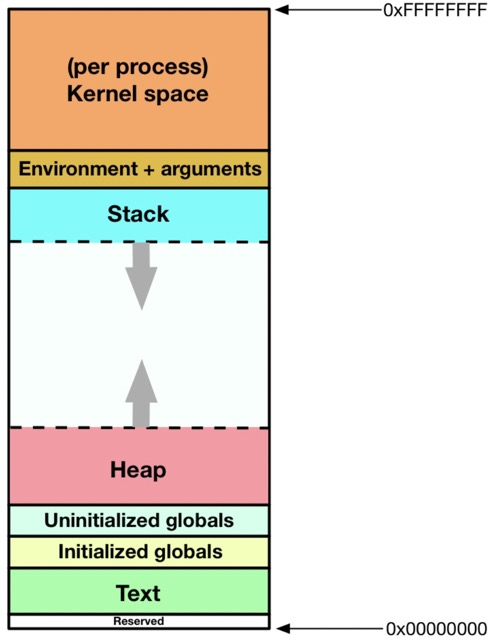
\includegraphics[scale=0.4]{virtmemproc.jpeg}
\caption{Memoria virtuale di un processo} 
\label{virtmemproc}
\end{figure}


Questa memoria (in questo per sistemi a 32bit) è suddivisa in:

\begin{itemize}
	\item \hl{Reserved}: parte riservata da 0 a n GB
	\item \hl{Text}: \textbf{codice eseguibile} del programma, utile al processore
	\item \hl{Initialized globals}: variabili dichiarate globali ed inizializzate
	\item \hl{Uninitialized globals}: 
	\item \hl{Heap}: parte alla quale ci si accede tramite delle richieste, per esempio con la malloc. Notare che la maggior parte di queste zone di memoria sono preallocate. Nell'heap ci finiscono anche le librerie dinamiche, dato che è codice di sola lettura. Queste sono allocate in modo randomico per rendere cmplicata la loro ricerca
	\item \hl{...}: spazio virtuale super mega ampio
	\item \hl{Kernel space}: zona vietata al programmatore dove il kernel fa le sue cose
	\item \hl{Environment + arguments}:
		\begin{itemize}
			\item \textbf{arguments}: stringhe passate al programma che le interpreterà
			\item \textbf{environment}: trovo i caratteri ASCII delle variabili di ambiente
		\end{itemize}
	\item \hl{Stack}: usato per \textbf{lavorare con le funzioni}, infatti quando una \textbf{funzione viene invocata mette in uno stack-frame le variabili locali} (o automatiche) allocate al momento della chiamata della funzione. Questa funzione potrebbe chiamarne un'altra, ecc ecc, allora lo \textbf{stack cresce verso il basso}. Ogni funzione può \textbf{accedere alle proprie variabili e a quelle globali}. È stata scelta questa organizzazione perché \textbf{non si può prevedere a priori quanto spazio servirà} perché potrebbe essere richiamata una funzione in modo ricorsivo, allora si usa lo \hl{swapping} e si fa di \textbf{non allocare nella RAM tutta la memoria del processo} ma solo quella necessaria. Il resto dei dati verranno pescati dalla memoria di massa tramite uno swap-in. 
\end{itemize}

Il massimo di dimensioni dello stack le vediamo da:

\begin{lstlisting}
$ ulimit -a

core file size          (blocks, -c) 0
data seg size           (kbytes, -d) unlimited
file size               (blocks, -f) unlimited
max locked memory       (kbytes, -l) unlimited
max memory size         (kbytes, -m) unlimited
open files                      (-n) 256
pipe size            (512 bytes, -p) 1
stack size              (kbytes, -s) 8192
cpu time               (seconds, -t) unlimited
max user processes              (-u) 709
virtual memory          (kbytes, -v) unlimited
\end{lstlisting}

di default sono a 8MB.

Per quanto riguarda il codice di ftw8.c (File Three Walk) sarà importante da padroneggiare per poter \hl{visitare tutti i nodi} a partire da una root decidendo, per ogni nodo, quale programma eseguire tramite una variabile \hl{Myfunc} creata da un typedef:

\begin{lstlisting}
typedef int     Myfunc(const char *, const struct stat *, int);
\end{lstlisting}

dove il tipo può assumere più valori da usare come \hl{coltellino svizzero}: 

\begin{itemize}
	\item \hl{FTW\_F}: ha uno switch annidato dove prende, da st\_mode, un campo della struttura attraverso un puntatore "->". Viene poi messo in "and" con una maschera per poter prendere il tipo di file sul quale fare i case
\end{itemize}

con questi case si potrà effettuare una statistica dei tipi di file nell'albero.

abremo anche:

\begin{itemize}
	\item \textbf{path\_alloc}: restituisce la massima dimenzione disponibile per un path in un determinato sistema operativo: PATH\_MAX + 1
\end{itemize}

in myftw la funzione dopath e1 ricorsiva e richiama se stessa per poter entrare nei nodi dell'albero

strcopy soggetta a stack overflow meglio usare strncopy

in fullpath avremo ttutti i path dei file da dare alla lstat() (lstat perchè ci serve che i link simboklici vengano visti come tali)

in dopath if 1 entra se in errore if 2 check se abbiamo una directory se non lo è fa un return perchè saremo arrivati alla foglia quindi torna indietro infatti FTW\_F if 3 se è una directory in ret = 0 e si continua 

notrare che pre far fermare la lettura si usa un 0 dato che null = 0 ma != "0"




chdir():
equivamente a cd, apssiamo un path e lui cambia cwd

fchdir():
fd si usa con open con flag per le direcotory

getcwd():
path abbastanza grande per path + null 



CAP 6

password file:
/etc/passwd in linux in mac sono se in modalità single user


uname():
dà le stesse info di uname -a


time and date routines:
sono le routine per fare il conto del tempo utile per il profiling di un programma dove si va a capire quando il programma ha tardato:
time() che ritorna il tempo in sec. funzione che da un valore assoluto con riferimento alle epoch. 
gettimeofday(): aggiunge i microsecondi quindi abbiamo unas truttura di 2 interi
clock\_gettime(): aggiugne i nanosec quindi abbiamo una struttura di 2 interi

questi secondi dono delle date infatti possiamo andare dai dec ad una struttra gmttime(): tempo del meridiano 0 localtime(): info sulla timezone. andiamo alloa ad una struttura tm che registra ore min sec ecc per fare in processo opposto usiamo mktime()



(sapere quando compiremo un miliardo di secondi)